\documentclass{article}
\usepackage[final]{neurips_2023}

\usepackage[utf8]{inputenc} % allow utf-8 input
\usepackage[T1]{fontenc}    % use 8-bit T1 fonts
\usepackage{hyperref}       % hyperlinks
\usepackage{url}            % simple URL typesetting
\usepackage{booktabs}       % professional-quality tables
\usepackage{amsfonts}       % blackboard math symbols
\usepackage{nicefrac}       % compact symbols for 1/2, etc.
\usepackage{microtype}      % microtypography
\usepackage{xcolor} 
\usepackage{graphicx}
\usepackage{float}
\usepackage{tabularx}
\usepackage{tikz}
\usepackage{empheq}
\usepackage{algorithm}
\usepackage{algpseudocode}  % or \usepackage{algorithmic}
\usepackage{xcolor}         % for coloring text
\usepackage{amsmath,amssymb}
\usepackage{fullpage}
\usepackage{bm}
\usepackage{tcolorbox}
\usepackage{float}
\usepackage{amsthm}
\usepackage{longtable}
\newtheorem{lemma}{Lemma}[section]
\theoremstyle{definition}
\newtheorem{definition}{Definition}
\newtheorem{theorem}{Theorem}[section]
\usepackage{longtable}




\title{Introduction to State Space Models}
\author{
\textbf{Vinay}\footnotemark[1] \quad
\textbf{Subhadeep Sing}\footnotemark[1] \quad
\textbf{Vaibhav Mahore}\footnotemark[1] \quad
\textbf{Snehal Biswas}\footnotemark[1] \\
\texttt{\{vinay2023, subh, vaibhav, snehal\}@iisc.ac.in} 
}
\begin{document}
\maketitle
\begin{abstract}
    This paper introduces \textbf{State Space Models} (SSMs) as a promising approach for sequential data modeling. We go through the fundamentals of SSMs, including their mathematical framework for describing dynamical systems through hidden states and observations. This paper details the \textbf{Linear State Space Layer} (LSSL) as a specific implementation. A core concept presented is the \textbf{High-Order Polynomial Projection Operators}  (HiPPO) framework, which efficiently compresses historical sequence data into a fixed-size representation using polynomial basis functions. This paper then explores the \textbf{Structured State Space for Sequence Modeling} (S4) model, highlighting its efficient parameterization and computation techniques, such as \textbf{Normal Plus Low-Rank} (NPLR) decomposition to handle the HiPPO matrix diagonalization challenges. Finally, it introduces the \textbf{MAMBA} architecture, which enhances SSMs with a \textbf{selection} mechanism, making parameters input-dependent to selectively compress context and overcome the limitations of time-invariant models, thereby improving performance on tasks requiring content-aware reasoning
\end{abstract}

\section{Introduction}
Sequence modeling aims to learn patterns or dependencies from data over time, mapping input $x(t)$ to output $y(t)$. Common approaches include RNNs, CNNs, and Transformers, each with unique trade-offs.

Ideally, we seek models that:
\begin{itemize}
    \item Support parallel training (like Transformers) with linear $O(N)$ complexity.
    \item Enable constant-time inference per token (like RNNs).
\end{itemize}

\textbf{State Space Models} (SSMs) emerge as a promising direction toward these goals.



\section{Methodology}
\subsection{SSMs}
A State Space Model (SSM) describes a dynamical system with a hidden state that evolves over time and an output dependent on that state, widely used in control theory and now in deep learning for modeling long-range dependencies in sequences.

\subsection{Linear State Spcae Layer(LSSL)}
\textbf{LSSL } is a \textbf{specific} way to implement SSMs. It is a simple sequence model that maps a 1-dimensional function or sequence $u(t) \rightarrow y(t)$ through a implicit state $x(t)$ by simulating a linear continuous time state space representation.
\[ \dot{x}(t) = A x(t) + B u(t), \quad y(t) = C x(t) + D u(t) \]


\subsection{Discretization of Continuous-Time Models}

In practice, because data is discrete (with \( u(t-\Delta t) \approx u(t) \)), we use the Generalized Bilinear Transform (GBT) to obtain the discrete state-space model:
\[
x_t = \bar{A}\,x_{t-1} + \bar{B}\,u_t,\quad y_t = Cx_t + Du_t,
\]
with
\[
\bar{A}=(I-\Delta t\,\alpha A)^{-1}[I+\Delta t\,(1-\alpha)A],\quad \bar{B}=(I-\Delta t\,\alpha A)^{-1}\Delta t\,B.
\]

Complete calculation and discussion of $\alpha$ is provided in Appendix~\hyperref[appendix:derivation of descritizatio]{[A1]}.


\subsection{LSSL: Recurrent and Convolutional Views}

\textbf{Recurrence.}  
Let \(x_{t-1} \in \mathbb{R}^{H \times N}\) represent the state. The update \(x_t\) and output \(y_t\) follow recurrence equations, making LSSL a recurrent model with constant per-step cost—suitable for autoregressive inference.

\textbf{Convolution.}  
The convolution kernel is defined as:
\[
K_L(\bar{A}, \bar{B}, \bar{C}) = \begin{bmatrix}
\bar{C}\bar{B}, & \bar{C}\bar{A}\bar{B}, & \dots, & \bar{C}\bar{A}^{L-1}\bar{B}
\end{bmatrix} \in \mathbb{R}^{H \times L},
\]
(see full derivation in Appendix~\hyperref[appendix:derivation of descritizatio]{[A1]}).

In this \textit{parallel} mode, the full input \(u = \{u_1, \dots, u_L\}\) is processed at once. Diagonalizing \(\bar{A}\) enables efficient FFT-based computation in \(\mathcal{O}(L \log L)\), ideal for fast, parallel training.



%hippo part
\subsection{High-Order Polynomial Projection Operators(HIPPO)}
\subsubsection{ Motivation}
Storing the full history of a continuous input stream \( f_t \) is impractical. The HiPPO framework addresses this by defining fixed matrices \( A \) (used in models like LSSL) that compress the past into a low-dimensional memory. This enables sequence modeling without retaining all previous data.

The core idea is \emph{function approximation using a probability measure}. A measure \( \mu \) on \( [0,\infty) \) defines an inner product \( \langle f, g \rangle_\mu = \int f(x)g(x)\,d\mu(x) \), turning function space into a Hilbert space with norm \( \|f\|_{L^2(\mu)} = \sqrt{\langle f, f \rangle_\mu} \). In this space, \( f_t \) is projected onto polynomial basis functions.



\subsubsection{HiPPO Abstraction and Memory Update}

The HiPPO framework enables online function approximation by projecting the input history \( f_t \) onto a polynomial subspace using a time-varying measure \( \mu_t \). It defines:

\begin{itemize}
  \item A \emph{projection operator} \( \operatorname{proj}_t \), which maps the restricted function \( f_t(x) = f(x) \) on \([0, t]\) to a polynomial \( g(t) \in \mathcal{G} \), minimizing the approximation error \( \|f_t - g(t)\|_{L^2(\mu_t)} \).
  \item A \emph{coefficient operator} \( \operatorname{coef}_t \), extracting a vector \( c(t) \in \mathbb{R}^N \) representing \( g(t) \) in an orthogonal polynomial basis.
\end{itemize}

The memory state \( c(t) \) evolves as \( \frac{d}{dt} c(t) = A_t c(t) + B_t f(t) \), discretized as \( c_{k+1} = A_k c_k + B_k f_k \), enabling efficient online compression of the input history.



We primarily use three HiPPO variants: \textbf{HiPPO-LegT, HiPPO-LagT, and HiPPO-LegS}.~\hyperref[appendix:Three type of hippo]{A1}



\subsection{Structured State Space for Sequence Modeling (S4)}
The \textbf{S4} model transforms a continuous SSM into a stable discrete recurrent or convolutional form using \textbf{NPLR} diagonalization and Cauchy-based kernel evaluation.

\subsubsection{Diagonalization of HiPPO Matrix A}
To overcome the bottleneck of repeated multiplications by $\bar{A}$ in the discrete-time SSM, we diagonalize $A$. This step is justified by the following:

\begin{lemma}
Conjugation is an equivalence relation on SSMs:
\[
(A,B,C) \sim (V^{-1}AV,\; V^{-1}B,\; CV) \quad \text{for any invertible matrix } V.
\]
\end{lemma}

Choosing $V$ such that $V^{-1}AV=\Lambda$ (diagonal) yields:
\[
A^k = V\,\Lambda^k V^{-1}, \quad K = CA^kB = CV\Lambda^kV^{-1}B.
\]
Since $\Lambda^k$ is trivial to compute, the sequence $\{\Lambda^k\}_{k=0}^{L-1}$ can be represented by a Vandermonde matrix. Fast polynomial transforms allow its multiplication in \(O((N+L)\log(N+L))\) time. However, because $V$ contains the eigenvectors of $A$, it is highly ill-conditioned.

\begin{lemma} The HiPPO matrix $A$ is diagonalized by a matrix $V$ with entries $V_{ij} = \binom{i+j}{i-j}$, which, for example, implies that $V_{3i,i}=\binom{4i}{2i}\approx2^{4i}$. Hence, $V$ can have entries up to roughly $2^{4N/3}$. \end{lemma}


\subsubsection{Normal Plus Low-Rank Decomposition}
To address the numerical instability of $V$, we conjugate using unitary (hence well-conditioned) matrices. Although the HiPPO matrix is not normal, it can be decomposed as the sum of a normal and a low-rank matrix:
\[
A = V\Lambda V^* - PQ^\top = V\Bigl(\Lambda - (V^*P)(V^*Q)^*\Bigr)V^*,
\]
where $V\in\mathbb{C}^{N\times N}$ is unitary, $\Lambda$ is diagonal, and $P,Q\in\mathbb{R}^{N\times r}$ with $r=1$ or $2$ (with equation (2) being $r=1$). Although exponentiating this sum is more challenging than diagonal matrices, the S4 paper presents three efficient techniques to handle it.



S4 performs convolution efficiently by using the Fourier transform instead of computing it directly in the time domain. The steps are:

\begin{enumerate}
 \item \textbf{Choose a length \(L\):}  
Truncate the kernel to length \(L\), since later terms often have minimal impact.

  \item \textbf{Transform to frequency domain and multiply:}  
Use FFT to convert both the input and kernel to the frequency domain, where convolution becomes fast elementwise multiplication, avoiding costly matrix operations.

  \item \textbf{Inverse FFT:}  
Apply IFFT to recover the final output in the time domain.

\end{enumerate}

This entire process only takes \(\mathcal{O}(L \log L)\) operations using FFT/IFFT, compared to the naive \(\mathcal{O}(N^2 L)\) time required for direct convolution involving matrix multiplications.For more detail Appendix~\hyperref[appendix:s4 algorithm]{A}




    
% Discuss related research, references, etc.

\subsection{Motivation for MAMBA: Selection as a Means of Compression}
The paper argue that a fundamental problem of sequence modeling is \textit{compressing context into a smaller state}. The paper propose \textbf{selectivity} as the fundamental principle for building sequence models. The selection mechanism is motivated using intuition from two synthetic task.

\begin{itemize}
    \item \textbf{Selective Copying}: The Selective Copying task modifies the popular Copying task (Arjovsky, Shah, and Bengio 2016) by varying the
    position of the tokens to memorize. It requires \textit{content-aware} reasoning to be able to memorize the relevant tokens
    (colored) and filter out the irrelevant ones (white).
    \item \textbf{Induction Head}: The Induction Heads task is a well-known mechanism hypothesized to explain the majority of in-context learning
    abilities of LLMs (Olsson et al. 2022). It requires \textit{context-aware}  reasoning to know when to produce the correct output in
    the appropriate context (black).

    \vspace{-5mm}
    \begin{figure}[H]
        \centering
        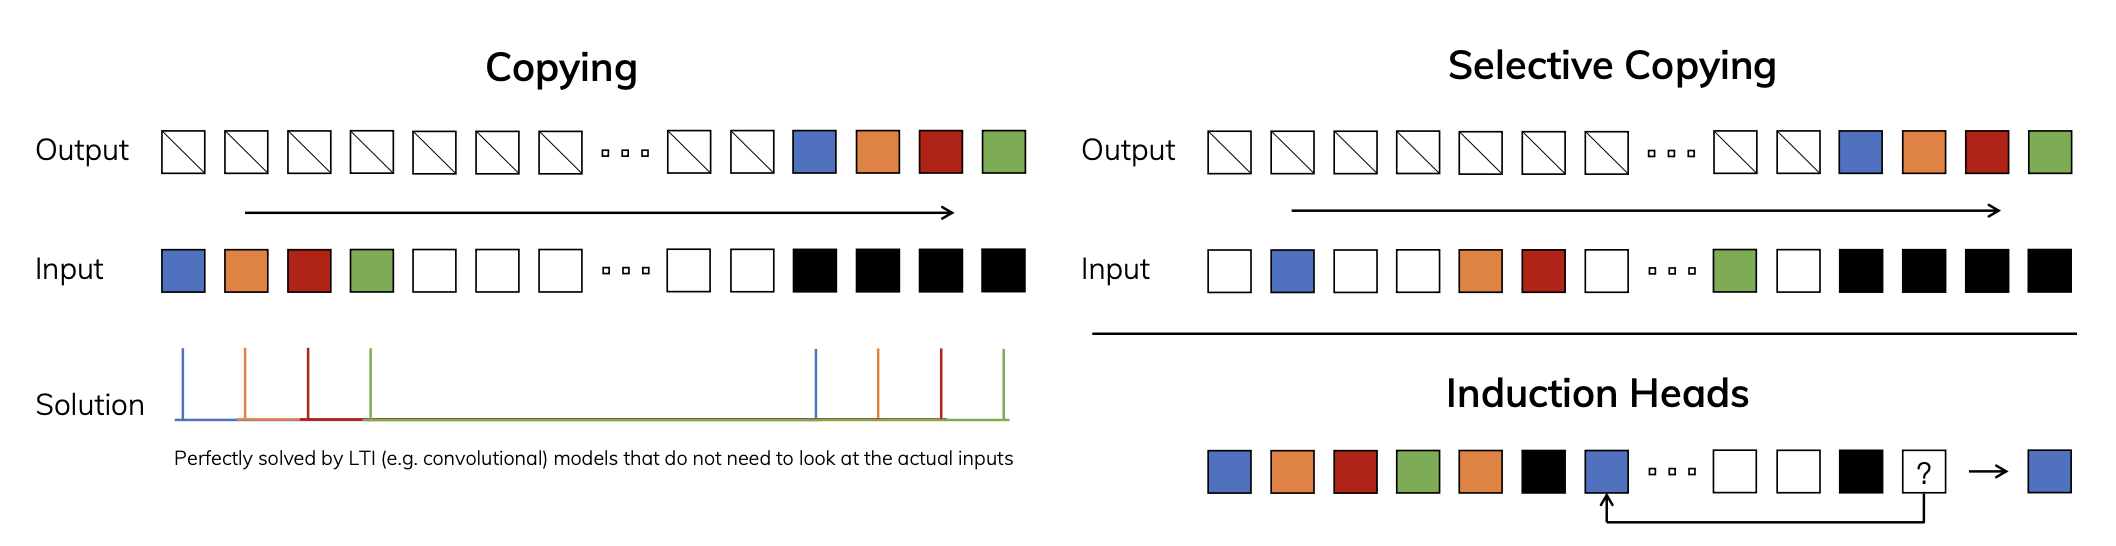
\includegraphics[scale=0.35]{synthetictask.png} % Replace with your actual image file name
       
        \label{fig:myimage}
    \end{figure}
\end{itemize}
  \vspace{-11mm}
  
\subsection{Selection Mechanism}
 \vspace{-17mm}
{\ttfamily
\begin{figure}[ht!]
    \centering
    \begin{minipage}[t]{0.48\textwidth}
    \begin{algorithm}[H]
    \caption{SSM (S4)}
    \label{alg:ssm-s4}
    \textbf{Input:} $x \colon (B,L,D)$ \\
    \textbf{Output:} $y \colon (B,L,D)$
    
    
    
    \begin{algorithmic}[1]
      \State \textbf{A}$ \colon (D, N)$ \hfill \(\leftarrow\) Parameter

      \medskip% Optional remark about the matrix

        \noindent \(\triangleright\) \emph{Represents structured $N \times N$ matrix}
    
      \State \textbf{B}$ \colon (D, N)$ \hfill \(\leftarrow\) Parameter
      \State \textbf{C}$ \colon (D, N)$ \hfill \(\leftarrow\) Parameter
      \State $\bm{\Delta}: \text{(D)} \leftarrow \tau_{\Delta}  \text{(Parameter)}$
      \State $\bar{\bm{A}} , \bar{\bm{B}}: \text{(D,N)} \leftarrow \text{discretize}(\bm{\Delta , A,B})$
      \State $\text{y} \leftarrow \text{SSM($\bar{\bm{A}} , \bar{\bm{B}} ,{\bm{C}}$)(x)}$
      \State  \hfill \(\triangleright\) Time-invariant: recurrence or convolution
      \State \textbf{return} $y$
    \end{algorithmic}
    \end{algorithm}
    \end{minipage}
    \hfill
    \begin{minipage}[t]{0.48\textwidth}
    \begin{algorithm}[H]
    \caption{SSM + Selection (S6)}
    \label{alg:ssm-s6}
    \textbf{Input:} $x \colon (B,L,D)$ \\
    \textbf{Output:} $y \colon (B,L,D)$
    
    
    
    \begin{algorithmic}[1]
      \State \textbf{A}$ \colon (D, N)$ \hfill \(\leftarrow\) Parameter

      \medskip% Optional remark about the matrix

        \noindent \(\triangleright\) \emph{Represents structured $N \times N$ matrix}
    
      \State \textbf{B}$ \colon (\textcolor{red}{B,L,N}) \leftarrow \textcolor{red}{s_B(x)} $ \hfill \(\leftarrow\) Parameter
      \State \textbf{C}$ \colon (\textcolor{red}{B,L,N}) \leftarrow \textcolor{red}{s_C(x)} $ \hfill \(\leftarrow\) Parameter
      
      \State $\bm{\Delta}: \textcolor{red}{B,L,D} \leftarrow \tau_{\Delta}  \text{(Parameter  \(\textcolor{red}{+ s_{\Delta}(x)}\))}$
      \State $\bar{\bm{A}} , \bar{\bm{B}}: \text{(B,L,D,N)} \leftarrow \text{discretize}(\bm{\Delta , A,B})$
      \State $\text{y} \leftarrow \text{SSM($\bar{\bm{A}} , \bar{\bm{B}} ,{\bm{C}}$)(x)}$
      \State  \hfill \(\triangleright\) \textcolor{red}{Time Varying}: recurrence \textcolor{red}{(scan)} only
      \State \textbf{return} $y$
    
    \end{algorithmic}
    \end{algorithm}
    \end{minipage}
    
    \end{figure}
}
\vspace{+2mm}
The main difference between \textbf{S4} and \textbf{MAMBA} is simply making several parameters $\Delta$  $\bm{ , B,C}$ functions of the input, along with the associated changes to tensor shapes throughout.
\begin{itemize}
   \item $\bm{s_B(x_t)} = \text{Linear}_N(x_t)$ computes token-specific $B_t$ from input $x_t$ via a linear layer.

    \item $\bm{s_C(x_t)} = \text{Linear}_N(x_t)$ computes token-specific output map $C_t$.

   \item $\tau_{\Delta} \; (\text{Parameter} + s_{\Delta}(x_t))$, where $s_{\Delta}(x_t) = \operatorname{Broadcast}_D(\operatorname{Linear}_1(x_t))$ is a learnable projection, and $\tau_{\Delta}$ (softplus) ensures a positive step size.


    \item The paper states that although \textbf{A} can be selective, it only influences the model via its interaction with $\Delta$ in $\bar{\textbf{A}} = \exp(\Delta \textbf{A})$, so selectivity in $\Delta$ is sufficient to ensure selectivity in $\bar{\textbf{A}}$, driving the main improvement.

\end{itemize}
The MAMBA \textbf{selection} algorithm can be nicely visualized with the picture given below:
\begin{figure}[H]
    \centering
    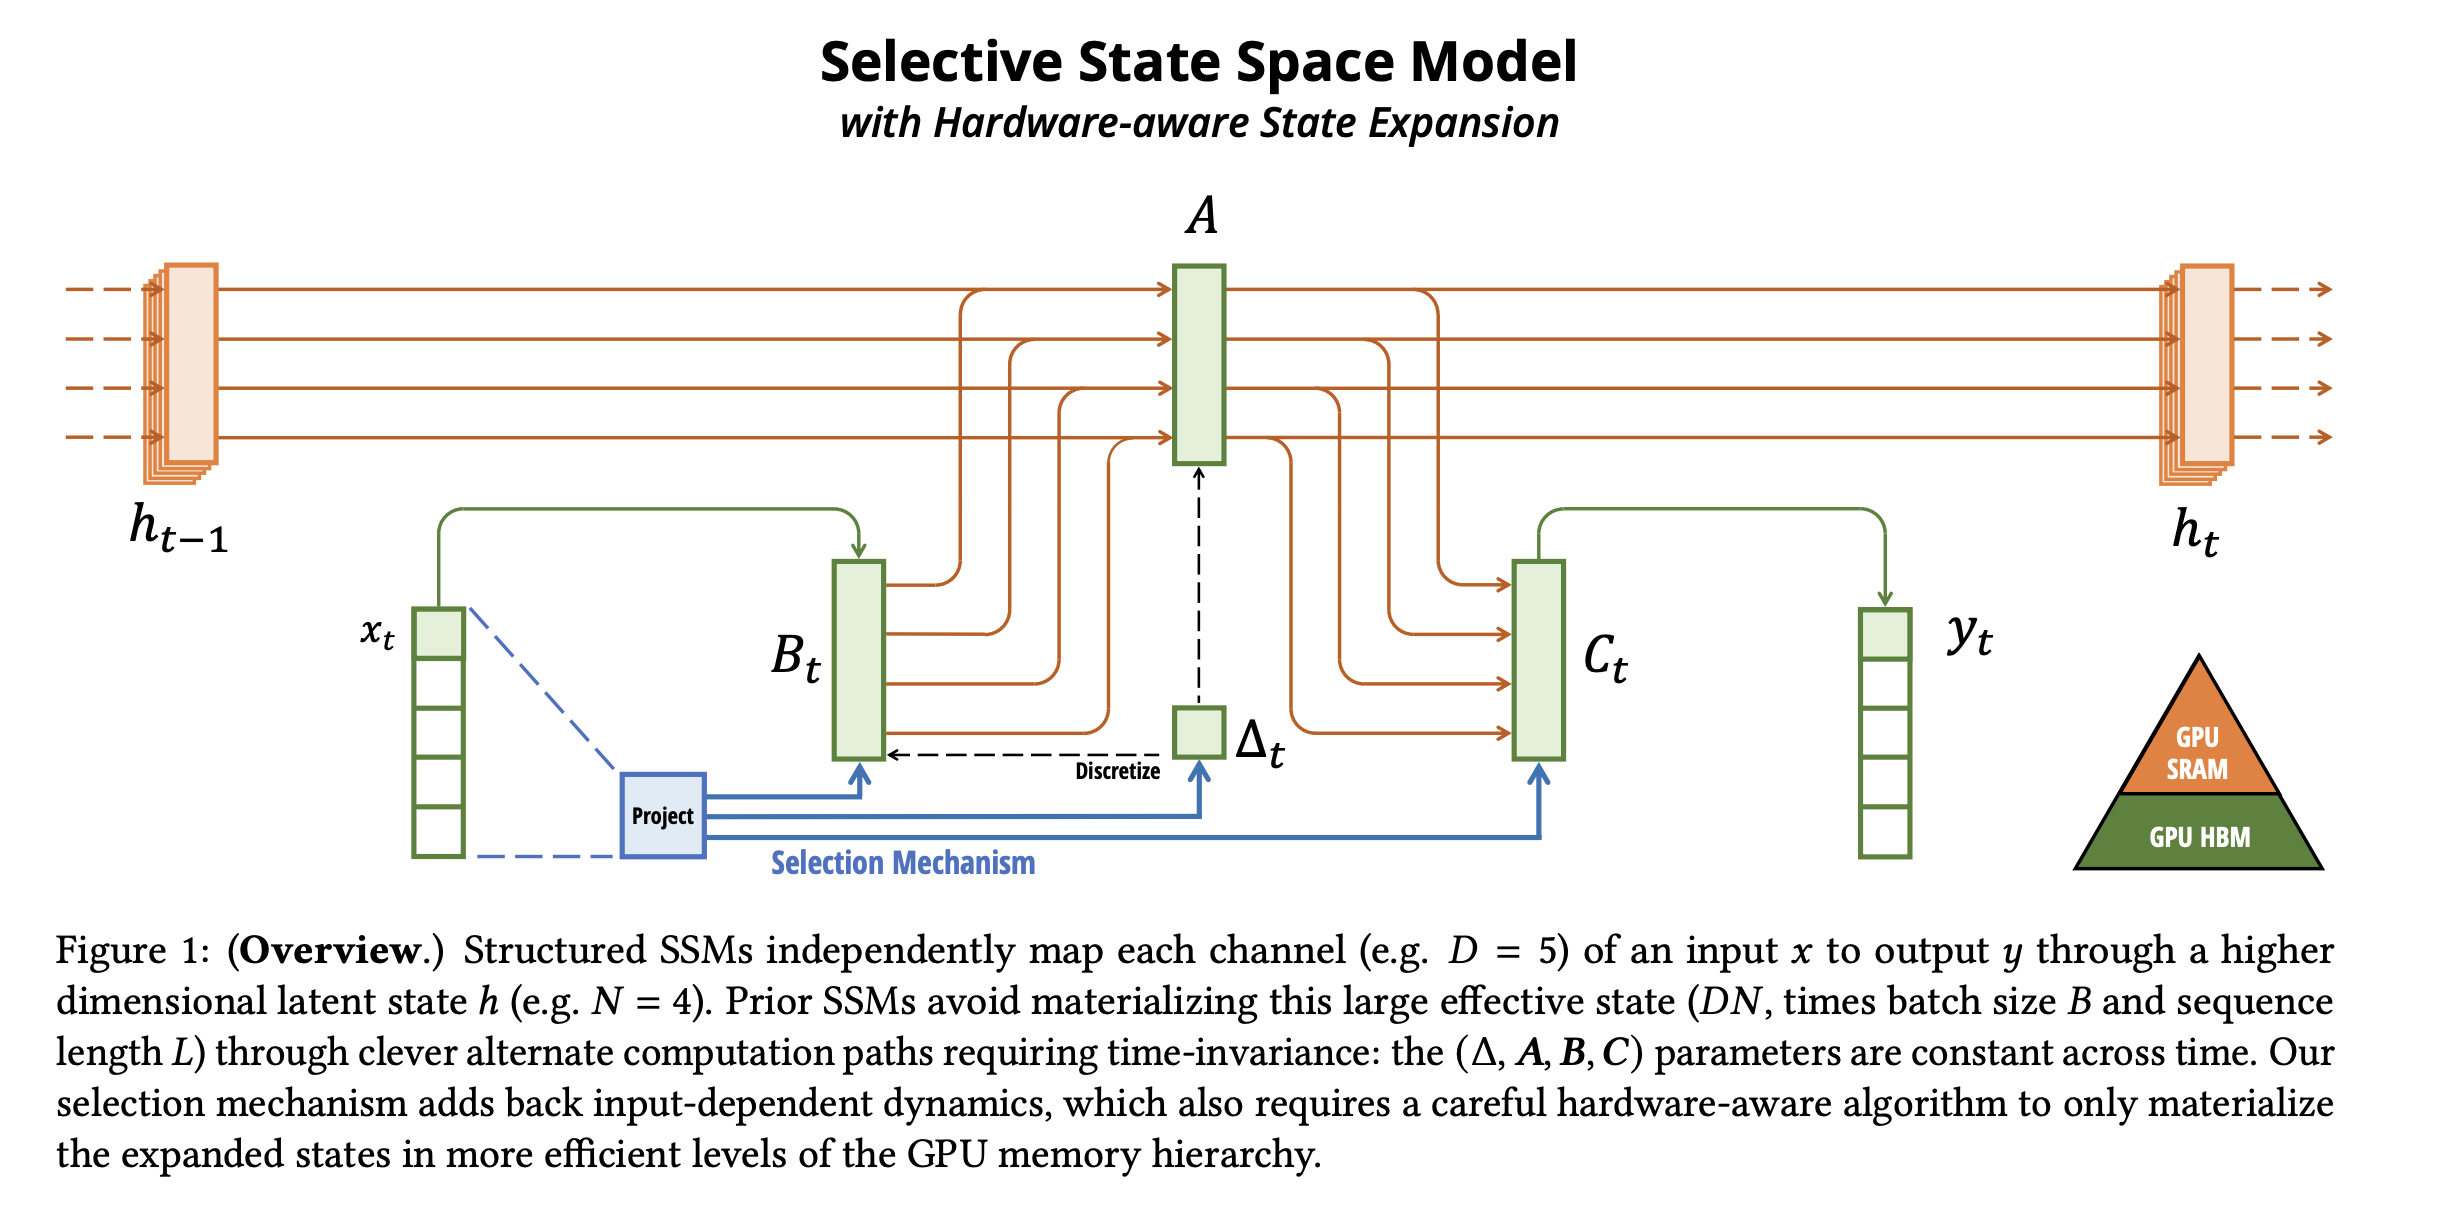
\includegraphics[width=1.0\textwidth]{image.png}
\end{figure}
A discussion on the selection mechanism's interpretation, gating connection, and its effects (variable spacing, context filtering, boundary resetting) is provided in Appendix~\hyperref[appendix:selection-mechanism]{[\ref*{appendix:selection-mechanism}]}.


\subsection{Overcoming Convolution Limitations in MAMBA}
Since MAMBA cannot be evaluated using a convolution(because it's time varying), it cannot be parallelized. Our only way to calculate it to use the recurrent formulation. The paper address this problem with three techniques: kernel fusion, parallel scan and recomputation. These techniques will \textbf{not} be discussed in this project paper.

\begin{thebibliography}{99}

\bibitem{gu2023combining}
Albert Gu, Isys Johnson, Karan Goel, Khaled Saab, Tri Dao, Atri Rudra, and Christopher Ré.
\newblock Combining Recurrent, Convolutional, and Continuous-time Models with Linear State-Space Layers.
\newblock In \textit{Proceedings of the Conference on Neural Information Processing Systems (NeurIPS)}, 2023.

\bibitem{gu2023hippo}
Albert Gu, Tri Dao, Stefano Ermon, Atri Rudra, and Christopher Ré.
\newblock HiPPO: Recurrent Memory with Optimal Polynomial Projections.
\newblock In \textit{Proceedings of the International Conference on Machine Learning (ICML)}, 2023.

\bibitem{gu2023efficiently}
Albert Gu, Karan Goel, and Christopher Ré.
\newblock Efficiently Modeling Long Sequences with Structured State Spaces.
\newblock In \textit{Proceedings of the Conference on Neural Information Processing Systems (NeurIPS)}, 2023.

\bibitem{gu2023mamba}
Albert Gu and Tri Dao.
\newblock Mamba: Linear-Time Sequence Modeling with Selective State Spaces.
\newblock In \textit{Proceedings of the Conference on Neural Information Processing Systems (NeurIPS)}, 2023.

\end{thebibliography}




\subsection

\section{Appendix}
\subsection{ Derivation of descritization}
\label{appendix:derivation of descritizatio}

The \textit{Generalized Bilinear Transform (GBT)} approximates the derivative and right-hand side using a weighted average.
\[
\dot{x}(t) \approx \frac{x(t) - x(t-\Delta t)}{\Delta t}
\]
Assuming \(u(t) \approx u(t-\Delta t)\) and letting \(\alpha \in [0,1]\), we write:
\[
\frac{x(t) - x(t-\Delta t)}{\Delta t} = (1 - \alpha)[Ax(t-\Delta t) + Bu(t)] + \alpha[Ax(t) + Bu(t)]
\]
Defining
\[
x_{t-1} = x(t-\Delta t), \quad x_t = x(t), \quad u_t = u(t),
\]
we have:
\[
\frac{x_t - x_{t-1}}{\Delta t} = (1 - \alpha) [Ax_{t-1} + Bu_t] + \alpha [Ax_t + Bu_t]
\]
Multiplying both sides by \(\Delta t\):
\[
x_t - x_{t-1} = \Delta t \left[(1 - \alpha)(Ax_{t-1} + Bu_t) + \alpha (Ax_t + Bu_t)\right]
\]
Rearrange the terms to isolate \(x_t\):
\[
x_t - \Delta t \alpha A x_t = x_{t-1} + \Delta t (1-\alpha)Ax_{t-1} + \Delta t B u_t
\]
Factorizing, we get:
\[
(I - \Delta t \alpha A)x_t = \big[I + \Delta t (1-\alpha)A\big]x_{t-1} + \Delta t B u_t
\]
Finally, solving for \(x_t\):
\[
x_t = (I - \Delta t \alpha A)^{-1}\left[\big(I + \Delta t (1-\alpha)A\big)x_{t-1} + \Delta t B u_t\right]
\]
\subsubsection{Role of \(\alpha\)}
\begin{itemize}
    \item \(\alpha = 0\) (Forward Euler):
    \[
    x_t = \Big(I + \Delta t\, A\Big)x_{t-1} + \Delta t\,B\, u_t.
    \]
    Simple but may be less stable.

    \item \(\alpha = 1\) (Backward Euler):
    \[
    x_t = \Big(I - \Delta t\, A\Big)^{-1}x_{t-1} + \Big(I - \Delta t\, A\Big)^{-1}\Delta t\,B\, u_t.
    \]
    Implicit formulation, which enhances stability.

    \item \(\alpha = 0.5\) (Trapezoidal):

  
    \[
    x_t = \left(I - \frac{\Delta t}{2}A\right)^{-1}\left[I + \frac{\Delta t}{2}A\right]x_{t-1} + \left(I - \frac{\Delta t}{2}A\right)^{-1}\Delta t\,B\, u_t.
    \]
    This formulation balances stability and accuracy.
\end{itemize}


\subsection{Convolution in LSSL}
\label{appendix:Convolution in LSSL}
\textbf{Convolution.}  
Assume \(x_{-1} = 0\). Unrolling the recurrences yields
\[
y_k = \bar{C}\,\bar{A}^k\,\bar{B}\,u_0 + \bar{C}\,\bar{A}^{k-1}\,\bar{B}\,u_1 + \cdots + \bar{C}\,\bar{A}\,\bar{B}\,u_{k-1} + \bar{B}\,u_k + \bar{D}\,u_k,
\]
so the output can be written as a convolution:
\[
y = K_L(\bar{A}, \bar{B}, \bar{C}) \ast u + \bar{D}\,u,
\]
with convolution kernel defined by
\[
K_L(\bar{A}, \bar{B}, \bar{C}) = \begin{bmatrix}
\bar{C}\,\bar{B}, & \bar{C}\,\bar{A}\,\bar{B}, & \dots, & \bar{C}\,\bar{A}^{L-1}\,\bar{B}
\end{bmatrix} \in \mathbb{R}^{H \times L}.
\]


\subsection{Three HiPPO Operators: LegT, LagT, and LegS}
\label{appendix:Three type of hippo}

\subsubsection{Types of HiPPO Operators}

Different choices of the measure \(\mu_t\) lead to distinct operators. Here we describe three variants: LegT, LagT, and LegS. (Note: \(\theta\) below is assumed to be a defined parameter).

\subsubsection{LegT}

For a uniform (or strict) window measure
\[
\mu_t(x) = \frac{1}{\theta} \mathbf{1}_{[t-\theta, t]}(x)
\]

the LegT operator projects the history. Its continuous-time dynamics are given by
\[
\frac{d}{dt} c(t) = A\, c(t) + B\, f(t),
\]
with coefficients defined as
\[
A_{nk} = \frac{1}{\theta}
\begin{cases}
(-1)^{n-k} (2n+1), & \text{if } n \ge k, \\
(2n+1), & \text{if } n < k,
\end{cases}
\qquad
B_n = \frac{1}{\theta} (2n+1) (-1)^n.
\]
Discretizing (using, e.g., the bilinear transform or ZOH) yields the update:
\[
c_{k+1} = A\, c_k + B\, f_k.
\]

\subsubsection{LagT}

For an exponentially decaying window measure defined by
\[
    \mu^{(t)}(x) = e^{-(t-x)} \, \mathbb{I}_{(-\infty, t]}(x)
    \begin{cases}
    e^{x-t}, & \text{if } x \le t, \\
    0, & \text{if } x > t,
    \end{cases}
\]
the LagT operator emphasizes recent inputs more strongly. Its continuous formulation is
\[
\frac{d}{dt} c(t) = A\, c(t) + B\, f(t),
\]
where
\[
A_{nk} =
\begin{cases}
1, & \text{if } n \ge k, \\
0, & \text{if } n < k,
\end{cases}
\qquad
B_n = 1.
\]
The corresponding discrete update is:
\[
c_{k+1} = A\, c_k + B\, f_k.
\]

\subsubsection{LegS}

The LegS operator. Its dynamics are given by:
\[
\frac{d}{dt} c(t) = -\frac{1}{t} A\, c(t) + \frac{1}{t} B\, f(t),
\]
with the discrete version given by
\[
    c_{k+1} = \left(\mathrm{Id} - \frac{1}{k} A\right) c_k + \frac{1}{k} B\, f_k
\]

The entries of \(A\) and \(B\) are specified as:
\[
A_{nk} =
\begin{cases}
\sqrt{(2n+1)(2k+1)}, & \text{if } n > k, \\
n+1, & \text{if } n = k, \\
0, & \text{if } n < k,
\end{cases}
\qquad
B_n = \sqrt{2n+1}.
\]

\begin{theorem}[Properties of HiPPO-LegS]
The HiPPO-LegS operator satisfies:
%for s4
\subsection{How s4  compute kernal }
\label{appendix:s4 algorithm}


\begin{figure}[h]
    \centering
    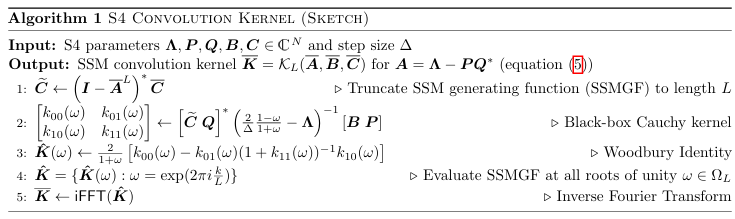
\includegraphics[width=\textwidth]{s4.png}
    
    \label{fig:myimage}
\end{figure}



\begin{itemize}
    \item Instead of computing $\overline{K}$ directly, we compute its spectrum by evaluating its \textbf{truncated generating function} $\sum_{j=0}^{L-1} K_j \zeta^j$ at the roots of unity $\zeta$. $\overline{K}$ can then be found by applying an inverse FFT.
    \item This generating function is closely related to the matrix resolvent, and now involves a matrix inverse instead of power. The low-rank term can now be corrected by applying the \textbf{Woodbury identity} which reduces $(A + PQ^*)^{-1}$ in terms of $A^{-1}$, truly reducing to the diagonal case.
    \item Finally, we show that the diagonal matrix case is equivalent to the computation of a \textbf{Cauchy kernel} $\frac{1}{\omega_j - \zeta_k}$, a well-studied problem with stable near-linear algorithms \cite{[30],[31]}.
\end{itemize}

Our techniques apply to any matrix that can be decomposed as \textbf{Normal Plus Low-Rank (NPLR)}.



\begin{enumerate}
  \item \textbf{Timescale Robustness:} It is equivariant to time dilation; rescaling the input function \( f \) does not affect the approximation coefficients.
  \item \textbf{Computational Efficiency:} Thanks to the triangular structure of \( A \), each discrete update is computable in \( O(N) \) operations.
  \item \textbf{Stable Gradient Propagation:} The \( \frac{1}{t} \) (or \( \frac{1}{k} \)) scaling ensures gradients remain stable, mitigating vanishing gradients.
\end{enumerate}
\end{theorem}
\subsection{Interpretation of Selection Mechanism}
\label{appendix:selection-mechanism}
\begin{itemize}
    \item \textbf{Connection to Gating Mechanism}: When we reduce the model to 1-Dimensional case i.e.  $N = 1$, $A = -1$, $B = 1$, $s_\Delta = \text{Linear}(x)$, and $\tau_\Delta = \text{softplus}$, then the selective SSM recurrence(Algorithm 2) takes the form
    \begin{align}
        g_t &= \sigma(\text{Linear}(x_t)) \hspace{16mm} (gate)\nonumber \\
        h_t &= (1 - g_t) h_{t-1} + g_t x_t  \hspace{7mm}  (update) \nonumber
    \end{align}

    \item \textbf{Variable Spacing}: Selectively filter out irrelevant or noisy tokens, such as language fillers, to focus on meaningful inputs.
    \item \textbf{Filtering Context}: Selectivity allows us to  dynamically reset the state and discard irrelevant historical information, allowing performance to improve consistently with increasing context length, unlike many traditional sequence models that struggle to ignore extraneous context.
    \item \textbf{Boundary Resetting}: In scenarios where multiple independent sequences are stitched togethere, Linear Time-invariant(LTI) models will bleed information between the sequences. Selective SSM's can  reset their state at boundaries (e.g $\Delta_t \rightarrow \infty$, or in gating when $g_t \rightarrow 1$).
\end{itemize}



\end{document}
